\documentclass[tikz]{standalone}

\usepackage{amsmath}
\usepackage{unicode-math}
\usepackage{mathtools}
\usepackage{derivative}

\setmainfont{Stix Two Text}
\setmathfont{Stix Two Math}

\usetikzlibrary{arrows.meta,fit,positioning}

\renewcommand{\familydefault}{\sfdefault}

% prefix equation numbers with section number
\numberwithin{equation}{section}

\DeclarePairedDelimiter{\ceil}{\lceil}{\rceil}
\DeclarePairedDelimiter{\floor}{\lfloor}{\rfloor}
\DeclarePairedDelimiter{\abs}{\lvert}{\rvert}
\DeclarePairedDelimiter{\norm}{\lVert}{\rVert}
\DeclarePairedDelimiter{\bra}{\langle}{\rvert}
\DeclarePairedDelimiter{\ket}{\lvert}{\rangle}
\DeclarePairedDelimiter{\expval}{\langle}{\rangle}
\DeclarePairedDelimiter{\norder}{\mathcolon}{\mathcolon}
\DeclarePairedDelimiter{\anorder}{\typecolon}{\typecolon}
	
\newcommand{\laplace}{\mbfnabla^2}
\newcommand{\trans}{{\scriptscriptstyle\mathsf{T}}}

\newcommand{\vdot}{\cdot}
\newcommand{\vcross}{\vectimes}
\newcommand{\vb}[1]{\symbfup{#1}}
\newcommand{\vu}[1]{\hat{\vb{#1}}}
\newcommand*\dd[2][\relax]{\mathop{\ifx\relax#1\odif{#2}\else \odif[order={#1}]{#2}\fi\,}}

\newcommand{\vacuum}{\ket*{\vb{0}}}

\DeclareMathOperator{\trace}{Tr}
\DeclareMathOperator{\sinc}{sinc}

\AtBeginDocument{
	\let\Re\relax
	\let\Im\relax
	\DeclareMathOperator{\Re}{Re}
	\DeclareMathOperator{\Im}{Im}

	\renewcommand{\div}{\mathop{\mbfnabla\vdot}}
	\newcommand{\curl}{\mathop{\mbfnabla\vectimes}}
}

\DeclarePairedDelimiterX{\comm}[2]{[}{]}{#1,#2}

\DeclarePairedDelimiterX{\braket}[2]{\langle}{\rangle}{#1\delimsize\vert#2}
\DeclarePairedDelimiterX{\ketbra}[1]{\lvert}{\rvert}{#1\rangle\delimsize\langle#1}



\begin{document}
	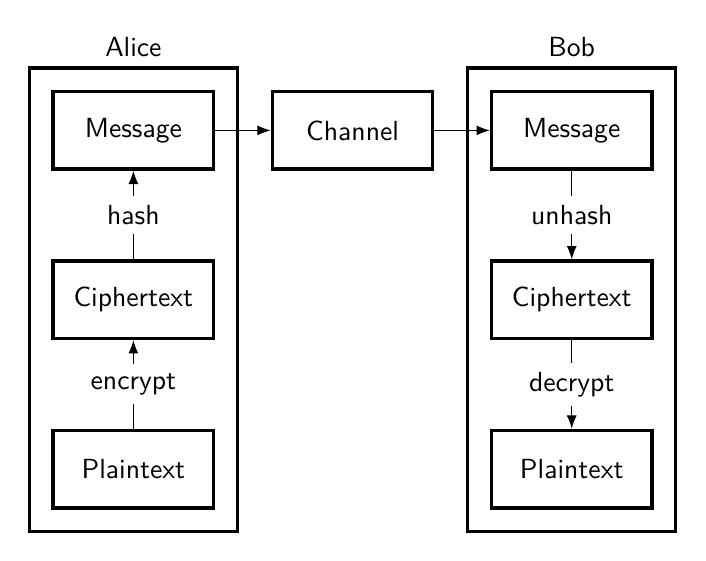
\begin{tikzpicture}[
		node distance=32pt,
		action/.style={midway, fill=white, align=center},
		block/.style={draw, very thick, fill=white, minimum height=28pt, minimum width=58pt},
		superblock/.style={draw, very thick, inner sep=8pt},
	]
		\coordinate (in) at (0,0);
		\node [block, above=of in] (plain a) {Plaintext};
		\node [block, above=of plain a] (cipher a) {Ciphertext};
		\node [block, above=of cipher a] (message a) {Message};
		\node [block, right=20pt of message a)] (channel) {Channel};
		\node [block, right=20pt of channel] (message b) {Message};
		\node [block, below=of message b] (cipher b) {Ciphertext};
		\node [block, below=of cipher b] (plain b) {Plaintext};
		\coordinate[below=of plain b] (out);
		
		\node [superblock, label={Alice}, fit=(plain a) (message a)] {};
		\node [superblock, label={Bob}, fit=(plain b) (message b)] {};
		
		\draw[-Latex] (plain a) -- (cipher a) node[action] (enc) {encrypt};
		\draw[-Latex] (cipher a) -- (message a) node[action] (hash) {hash};
		\draw[-Latex] (message a) -- (channel);
		\draw[-Latex] (channel) -- (message b);	
		\draw[-Latex] (message b) -- (cipher b) node[action] (unhash) {unhash};		
		\draw[-Latex] (cipher b) -- (plain b) node[action] (dec) {decrypt};
	\end{tikzpicture}
\end{document}
